\documentclass[a4paper,12pt]{article}
\usepackage[dvipsnames]{xcolor}
\usepackage[spanish, provide=*]{babel}
\usepackage[
  colorlinks=true, 
  linkcolor=black,
  pdfpagemode=FullScreen,
  pdftitle={Easycab}
]{hyperref}
\usepackage{graphicx}
\usepackage{adjustbox}

\usepackage{listings}
\usepackage{xcolor}
\usepackage{xcolor}
\usepackage{titling}
\usepackage{fontspec} % Para fuentes personalizadas (usar XeLaTeX o LuaLaTeX)
% \usepackage{minted}

\setmainfont{Kanit}
\setmonofont{CaskaydiaCove Nerd Font Mono}

\lstset{ 
  numbers=none,              % Numeración de líneas a la izquierda
  rulecolor=\color{black},   % Color de la línea de borde
}

\definecolor{mygreen}{rgb}{0,0.6,0}
\definecolor{myblue}{rgb}{0.1171875, 0.3984375, 0.95703125}
\definecolor{mymauve}{rgb}{0.53125, 0.22265625, 0.93359375}
\definecolor{mygray}{rgb}{0.296875, 0.30859375, 0.41015625}

\lstset{ %
  language=C,                
  basicstyle=\ttfamily\footnotesize,       
  backgroundcolor=\color{white},   
  breaklines=true,                 
  commentstyle=\color{mygray},    
  keywordstyle=\color{mymauve},       
  stringstyle=\color{mygreen},     
  frame=single,          
  showstringspaces=false,
  rulecolor=\color{black}, 
}

\title{Easycab}
\author{Aarón Blasco Tremiño \and (74379762Q)}
\date{\today}
 


\pretitle{\begin{center}\Huge\color{black}}
\posttitle{\end{center}}
\sloppy


\begin{document}

\maketitle

\clearpage
\hypersetup{linkcolor=black, urlcolor=cyan}
\tableofcontents  % Generates the table of contents with clickable links
\hypersetup{linkcolor=blue, urlcolor=blue, filecolor=cyan}
\clearpage

\section{Introducción}
\subsection{¿Qué es Easycab?}
Este proyecto implementa un sistema distribuido que simula una empresa
de taxis autónomos. En el sistema, diferentes clientes pueden pedir
servicios a diferentes puntos de la ciudad preestablecidos.
% TODO: Refinar, no es muy claro

\subsection{Enfoque y estructura de carpetas}
Este proyecto se ha desarrollado principalmente en C y utiliza \textit{cmake} como herramienta de construcción.
Para facilitar su portabilidad y acceso, todo el proyecto está disponible en un
\href{https://github.com/abtb2-ua/easycab}{repositorio público en GitHub}. A continuación, se presenta una breve
descripción de la estructura de carpetas:

\begin{itemize}

  \item La carpeta \textbf{src} contiene todo el código fuente del proyecto, incluyendo los archivos de cabecera
        (\textit{.h}) y sus implementaciones (\textit{.c}). También se encuentra el script
        \textit{\href{https://github.com/abtb2-ua/easycab/blob/main/src/initialize.sql}{initialize.sql}}, que se
        utiliza para inicializar la base de datos. Además, esta carpeta incluye el symlink
        \textit{\href{https://github.com/abtb2-ua/easycab/blob/main/src/compile_commands.json}{compile\_commands.json}},
        que apunta a un archivo generado automáticamente al compilar con \textit{cmake}. Este archivo es útil únicamente
        para el desarrollo, ya que facilita las sugerencias de código en \textit{clangd}.

  \item La carpeta \textbf{res} contiene los archivos de texto necesarios para que \break\textit{EC\_Customer} y \textit{EC\_Central}
        lean los servicios a solicitar y las ubicaciones del mapa, respectivamente. Estos archivos se emplearon durante el desarrollo
        para realizar pruebas del sistema.

  \item En \textbf{docs} se encuentra la documentación del proyecto en formato LaTeX, tanto el código fuente como el archivo PDF generado.

  \item La carpeta \textbf{visual studio} alberga el subproyecto de Visual Studio que sirve como portabilidad para la interfaz gráfica
        en Windows. Esto se debe a que la dockerización de la interfaz gráfica resulta algo compleja, por lo que se optó por migrarla a
        un entorno nativo de Windows para facilitar su uso. Alternativamente, se puede compilar la versión con \textit{cmake} descomentando
        el contenido correspondiente en el archivo
        \textit{\href{https://github.com/abtb2-ua/easycab/blob/main/CMakeLists.txt}{CMakeLists.txt}} y asegurándose de contar con la librería
        \textit{raylib}.

  \item La carpeta \textbf{.vscode} contiene únicamente el archivo de configuración
        \textit{\href{https://github.com/abtb2-ua/easycab/blob/main/.vscode/settings.json}{settings.json}} para el editor \textit{VSCode}.
        Este archivo configura la extensión \textit{Material Icon Theme}, de carácter estético.

  \item Finalmente, en la carpeta \textbf{raíz} se ubican los archivos de configuración del proyecto y del repositorio,
        como \textit{\href{https://github.com/abtb2-ua/easycab/blob/main/.gitignore}{.gitignore}} y \textit{\href{https://github.com/abtb2-ua/easycab/blob/main/CMakeLists.txt}{CMakeLists.txt}}. \end{itemize}

\subsection{Herramientas utilizadas}
\begin{itemize}
  \item \textbf{Visual Studio Code} y \textbf{Visual Studio 2019} como editores de código.
  \item \textbf{CMake} como sistema de compilación.
  \item \textbf{Git} como sistema de control de versiones.
  \item \textbf{Docker} para facilitar el despliegue.
  \item \textbf{Raylib} como librería para la interfaz gráfica.
  \item \textbf{Mysql Server} como sistema de gestión de base de datos.
  \item La librería \textbf{Ncurses} para implementar la interfaz gráfica en terminal.
  \item Las librerías \textbf{rdkafka}, \textbf{mysqlclient}, \textbf{uuid} y \textbf{glib} para el desarrollo general del proyecto
\end{itemize}

\subsection{Componentes del sistema}
\begin{itemize}
  \item \textbf{EC\_Central}: Componente angular del sistema, se encarga de la comunicación con los clientes y los taxis.
        Consiste en 3 módulos (sin incluir el entrypoint \textit{EC\_Central.c}):
        \begin{itemize}
          \item \textbf{kafka\_module}: Módulo que se encarga de la comunicación con los clientes y los taxis a través de Kafka.
          \item \textbf{ncurses\_gui}: Módulo que se encarga de la interfaz gráfica (en terminal) de la central.
          \item \textbf{socket\_module}: Módulo que se encarga de la autenticación de los taxis via sockets.
        \end{itemize}
  \item \textbf{EC\_DE}: Representa el software central de un taxi autónomo. Recibe instrucciones de la central y se mueve por
        el mapa independiente e asíncronamente del resto de taxis. Este componente también incluye el módulo \textbf{EC\_DE\_ncurses\_gui}
        que se encarga de la interfaz gráfica (en terminal) del taxi.
  \item \textbf{EC\_SE}: Representa el sensor de un taxi autónomo. Este componente es dependiente de EC\_DE, con el cual se comunica
        a través de sockets para informar sobre la situación del taxi.
  \item \textbf{EC\_Customer}: Representa a un cliente. Su única fución en el sistema es pedir servicios a la central continuamente.
  \item \textbf{Interfaz gráfica (gui)}: Lee las comunicaciones en kafka y muestra la información en forma de ventana. Como se ha comentado anteriormente,
        este componente tiene dos implementaciones en el proyecto, una en \textbf{src}, basada en un entorno de Linux; y otra en
        \textbf{visual studio}, basada en Windows. Puesto que su implementación en Linux se ha probado menos exhaustivamente, se
        recomienda el uso de la implementación en Windows.
\end{itemize}

\clearpage
\section{Implementación}
\subsection{Cabeceras comunes}
En el desarrollo de este proyecto he hecho uso de varias cabeceras comunes entre varios de los componentes. Estas cabeceras
contienen funciones y estructuras de datos que son utilizadas en el resto del proyecto y que, en muchos casos, es importante
que sean iguales en todos los componentes.
\subsubsection{Common}
Contiene el grueso de las definiciones y funciones comunes en el proyecto. Repasémoslas brevemente:
\begin{itemize}
  \item Al comienzo de la cabecera podemos hayar algunas definiciones de constantes y enumeraciones que, puesto que son simples y están debidamente comentadas,
        ignoraré aquí. No obstante, recomiendo echarles un vistazo en el \href{https://github.com/abtb2-ua/easycab/blob/main/src/common.h}{código fuente}. \par
        El único que me parece merecedor de mención es el enum \textbf{SUBJECT}. La mayoría de las comunicaciones en este proyecto se definen por un
        \textit{motivo} (el cómo se usa, se irá viendo a lo largo de la memoria). De esta manera, podemos categorizar las comunicaciones de manera clara y atenderlas ordenadamente.
        De nuevo, como es un enum largo (así lo es la cantidad de razones por las que los diferentes componentes pueden querer comunicarse entre ellos)
        y sus valores son razonablemente autoexplicativos, evitaré ensuciar el documento con el código.
  \item Continuamos con las estructuras de datos que usarán ampliamente durante el proyecto:
        \begin{lstlisting}[language=C]
// Position in the map
typedef struct {
  int x, y;
} Coordinate;

// Represents a socket address
typedef struct {
  char ip[20];
  int port;
} Address;
        \end{lstlisting}
        \par
        Estas estructuras son muy simples y, como se puede ver, no requieren comentarios. Simplemente organizan los datos para una mayor legibilidad.
  \item \begin{lstlisting}[language=C]
// Represents an entity relevant for the progress of the system
typedef struct {
  ENTITY_TYPE type;      // Customer, taxi or location
  USER_STATUS status;    // Unset if the entity is a location
  Coordinate coord;      // Position in the map
  int id;                // Represents a char if the entity is not a taxi
  char obj;              // Customer's destination or taxi's service
  bool carryingCustomer; // Only for taxis
} Entity;
        \end{lstlisting}
        Este struct representa o bien una localización, un cliente o un taxi y contiene toda la información relevante para que las interfaces gráficas
        puedan representarlos adecuadamente. Nótese que no todos los valores del struct son usados para todos los tipos de entidad. Por ejemplo,
        \textit{obj} no tiene sentido en caso de una localización y \textit{carryingCustomer} sólo es relevante para los taxis. \par
        La razón de que exista un único struct para representar todos los tipos de entidad es la organización y poder normalizar las comunicaciones.
        De esta manera, tanto los remitentes como los destinatarios de la información siempre manejan la misma cantidad de datos y podemos evitar los
        accesos fuera de rango tan característicos de c.
  \item \begin{lstlisting}[language=C]
// Represents a message sent by a user to the central
typedef struct {
  SUBJECT subject;           // Purpose of the message
  Coordinate coord;          // Position of the author (may be unused)
  int id;                    // Identification of the author
  char data[UUID_LENGTH];    // Extra data, depending on the subject
  char session[UUID_LENGTH]; // Session id of the system, restarted each time the system restarts.
                             // Its possition as last in the struct is relevant, don't change it
} Request;

// Represents a message sent by the central to a user
typedef struct {
  SUBJECT subject;           // Purpose of the message
  int map[MAP_SIZE];         // 100 (taxis) + 30 (customers) + 30 (locations)
                             // Represents the state of the map
  char id;                   // Identification of the addressee
  char data[UUID_LENGTH];    // Extra data, depending on the subject
  char session[UUID_LENGTH]; // Session id of the system, restarted each time the system restarts.
                             // Its possition as last in the struct is relevant, don't change it
} Response;
        \end{lstlisting}
        Por el mismo motivo que antes, todas las comunicaciones tienen la misma estructura y, por tanto, la misma cantidad de datos. Así pues, Request
        representará un mensaje enviado a través de kafka \underline{hacia} la central y Response uno enviado \underline{desde} la central. \par
        Como se explicó anteriormente, tanto las requests como las responses se caracterizan por un \textit{subject} o \textit{motivo}. También
        contienen, como era de esperar, el id del remitente/destinatario y un campo para añadir datos adicionales si es necesario. \par \break
        Es interesante mencionar que el mapa se envía como un \break array de enteros porque cada uno representa un \textbf{Entity} serializado.
        Aprovechamos el hecho de que la mayoría de sus campos no necesitan mucho del espacio que ocupan (como los valores \textbf{Coordinate},
        ue a lo largo del programa solo adoptarán valores del 0 al 20) y logramos reducir el espacio del mapa y el peso de las comunicaciones considerablemente.\par
        Por último, el campo \textbf{session} juega un papel importante. Cada vez que el sistema se reinicia, crearemos una nueva sesión con un id único.
        Así, todos los componentes podrán descartar mensajes que no sean relevantes y puedan generar líos entre ellos. Por ejemplo, si se nos ha olvidado
        cortar la ejecución de un taxi antes de reiniciar la bbdd, sin la ayuda de \textbf{session} la central podría estar tratando de mover un taxi que realmente
        no existe en la base de datos. Si bien no tiene por qué ser necesario si el sistema es robusto, no sobra tomar precauciones.
  \item Gestión de logs:
        \begin{lstlisting}[language=C]
void log_handler(const gchar *log_domain, GLogLevelFlags log_level, const gchar *message,
        gpointer user_data);
        \end{lstlisting}
        Esta función redefine los el formato de los mensajes de la librería \textbf{glib}. Así pues, podemos usar su API:
        \begin{lstlisting}[language=C]
g_log_set_handler(NULL, G_LOG_LEVEL_DEBUG, log_handler, NULL);

g_message("This is a message");
g_warning("This is a warning");
g_error("This is an error");
g_critical("This is a critical error");
g_debug("This is a debug message");
        \end{lstlisting}
        Con un formato más acorde al estilo del proyecto (y al mío personal).
        \begin{figure}[h]
          \centering
          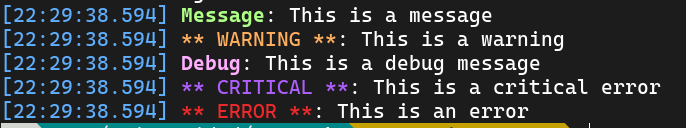
\includegraphics[width=1\textwidth]{img1.png}
          \caption{Ejemplo de ejecución de mensajes a través de la API de glib.}
          \label{fig:ejemplo}
        \end{figure}
  \item Serialización de entidades:
        \begin{lstlisting}[language=C]
int serializeEntity(Entity *entity);
void deserializeEntity(Entity *dest, int entity);
        \end{lstlisting}
        Como se comentó anteriormente, ambas funciones aprovechan el hecho de que los campos de \textbf{Entity} no necesitan todo el espacio que ocupan
        para almacenar sus datos en el tamaño de 4 bytes.
  \item Funciones comunes sobre sockets:
        \begin{lstlisting}[language=C]
int openSocket(int port);
int connectToServer(Address *server);
\end{lstlisting}
        Estas funciones hacen lo que prometen y nada más: abrir un socket servidor o conectarse a uno, devolviendo en ambos casos el descriptor de socket
        correspondiente. Además, se encargan de manejar errores y asignar una rutina de cierre de socket al cierre del programa.
  \item Funciones comunes sobre kafka:
        \begin{lstlisting}[language=C]
rd_kafka_t *createKafkaUser(Address *server, rd_kafka_type_t type, char *id);
void subscribeToTopics(rd_kafka_t **consumer, const char **topics, int topicsCount);
void sendEvent(rd_kafka_t *producer, const char *topic, void *value, size_t valueSize);
rd_kafka_message_t *poll_wrapper(rd_kafka_t *rk, int timeout_ms);
\end{lstlisting}
        Las dos primeras funciones son similares a las del apartado anterior, en el sentido de que inicia la comunicación pero en este caso, con kafka. Es importante
        mencionar que es posible usar \textbf{createKafkaAgent} para crear un producer o un consumer, únicamente cambiando el segundo parámetro. La segunda función,
        sin embargo, solo tiene sentido para un consumer. \par
        Las últimas dos funciones son simplemente envoltorios de las funciones para enviar o recibir mensajes con la finalidad de mejorar la legibilidad del código.
        La única funcionalidad un tanto especial es la de \textbf{poll\_wrapper} que solo devuelve los mensajes enviados después de la
        marca de tiempo determinada (relativa al momento actual). Esto se puede hacer porque la key de todos los mensajes enviados
        es la fecha de envío en formato \textit{UNIX} \par
        Algo que quizá sí que es merecedor de mención es la configuración con que se inicializan los consumers/producers:
        \begin{lstlisting}[language=C]
SET_CONFIG(conf, "log_level", "0", errstr);
SET_CONFIG(conf, "bootstrap.servers", serverAddressStr, errstr);
SET_CONFIG(conf, "client.id", id, errstr);
SET_CONFIG(conf, "acks", "all", errstr);
SET_CONFIG(conf, "auto.offset.reset", "earliest", errstr);
if (type == RD_KAFKA_CONSUMER) {
  SET_CONFIG(conf, "group.id", id, errstr);
  SET_CONFIG(conf, "session.timeout.ms", "6000", errstr);
  SET_CONFIG(conf, "max.poll.interval.ms", "6000", errstr);
}
        \end{lstlisting}
        Nótese que las variables id y serverAddressStr son las pasadas por parámetro (y una traducción de Address a string en caso de la segunda).
        mientras que la primera configuración puede no ser muy relevante para la ejecución del sistema, el resto sí lo son. Su intención es
        asegurar que las comunicaciones se realizan de un modo seguro (\textit{acks=all}) y que no se pierdan mensajes (\textit{auto.offset.reset=earliest}).
        No obstante, esta última no significa que cada vez que se cree un consumer empieze realmente a leer desde el principio del topic. Puesto que en la mayoría
        de casos se crean siempre con la misma id, esta configuración solo significa que retomarán la lectura desde donde lo dejaron. Con respecto a las dos últimas
        configuraciones, tienen los valores mínimos para que los consumers/producers expiren tan pronto como sea posible si no se les ha cerrado
        explícitamente mediante código.
\end{itemize}
\subsubsection{Estructuras de datos}
Este archivo contiene un par de estructuras de datos simples que yo mismo he desarrollado:
\begin{itemize}
  \item \textbf{TABLE}: Representa literalmente una tabla con la intención de ser impresa en una interfaz gráfica. Puesto que
        no es relevante para el funcionamiento del sistema, no profundizaremos en ella. Esta es su API:
        \begin{lstlisting}[language=C]
/// @brief Initializes a table
///
/// @param table Table to be initialized
/// @param start Coordinate where the table will start (top left corner)
/// @param title Title of the table
/// @param headers Array of strings that will be used as headers
/// @param headers_num Number of headers
/// @param err_color Color in which the rows will be printed if set as erroneous
void initTable(Table *table, Coordinate start, char *title, char **headers, int headers_num,
                int err_color);

/// @brief Prints a table in a ncurses window
///
/// @param table Table to be printed
/// @param win Window in which the table will be printed
void printTable(Table *table, WINDOW *win);

/// @brief Adds a row to a table
///
/// @param table Table to which the row will be added
/// @param row Array of strings that will be used as row's content
/// @param status Whether the row is erroneous or not (if erroneous, the row will be printed in
/// a different color)
void addRow(Table *table, const char **row, bool status);

/// @brief Deletes all the rows from a table
///
/// @param table Table to be emptied
void emptyTable(Table *table);

/// @brief Disposes the memory allocated for a table
///
/// @param table Table to be destroyed
void destroyTable(Table *table);
        \end{lstlisting}
  \item \textbf{QUEUE}: Representa una cola FIFO, otra vez usada únicamente en las interfaces gráficas de terminal. No hay mucho que explicar sobre ella, esta es su API:
        \begin{lstlisting}[language=C]

/// @brief Returns a new queue
///
/// @return Queue* Empty queue
Queue *newQueue();

/// @brief Initializes a queue iterator
///
/// @param queue Queue to be iterated
/// @return QueueIterator Iterator to be used
QueueIterator initQueueIterator(Queue *queue);

/// @brief Gets the next element in the queue
///
/// @param queue Queue to be iterated
/// @param it Iterator to be used
/// @param element Pointer to the element to be filled
/// @return true There is an element to be read
/// @return false There aren't anymore elements to be read
bool getNext(Queue *queue, QueueIterator *it, void *element);

/// @brief Pops the first element in the queue (if queue is not empty)
///
/// @param queue Queue to be iterated
/// @param element Pointer to the element to be filled
/// @return true There is an element to be popped
/// @return false The queue is empty
bool dequeue(Queue *queue, void *element);

/// @brief Pushes an element in the queue. If the queue is full, the oldest element will be
/// popped
///
/// @param queue Queue to be iterated
/// @param element Pointer to the element to be pushed
void enqueue(Queue *queue, void *element);
        \end{lstlisting}
        Nótese que pueden faltar algunas funciones características de colas. Esto es porque solo se han
        definido las funciones que se necesitan para el funcionamiento del sistema.
\end{itemize}
\subsubsection{Funciones comunes de Ncurses}
Al igual que el data\_structures.h, este archivo contiene fucniones exclusivamente relevantes para las interfaces gráficas de terminal
(implementadas con la librería \textbf{ncurses}). Continuando con la tónica de no profundizar en lo relativo con las interfaces gráficas,
he aquí la API de su cabecera:
\begin{lstlisting}[language=C]
/// @brief Initializes a 256-based rgb color in the ncurses palette
///
/// @param color Color to be initialized
/// @param r Red component
/// @param g Green component
/// @param b Blue component
void init_color_rgb(int color, int r, int g, int b);

/// @brief Prepares the ncurses GUI for the use of colors (e.g. initializing the palette)
void start_color_wrapper();

/// @brief Handles the logging of the ncurses GUI through the glib API
void ncurses_log_handler(const gchar *log_domain, GLogLevelFlags log_level, const gchar *message,
                          gpointer user_data);

/// @brief Prints a pop-up message informing the user that the program is exiting
///
/// @param extra Extra message to be printed, if NULL, no more than the default message will be
/// printed
void printFinishPopUp(char *extra);

/// @brief Finds a character in a string
///
/// @param text String to be searched
/// @param character Character to be found
/// @return int Position of the character in the string or -1 if not found
int find(const char text[], char character);

/// @brief Splits a string into lines of a given length without breaking words
///
/// @param dest Array of strings where the lines will be stored
/// @param text String to be split
/// @param lineLength Maximum length of each line
/// @return int Number of lines
int split(void *dest, const char text[], int lineLength);
\end{lstlisting}
\subsection{EC\_Customer}
Comencemos con "la chicha" del proyecto. El componente EC\_Customer es probablemente el más pequeño y sencillo de los componentes.
Su flujo de ejecución es el siguiente:
\begin{enumerate}
  \item Se comprueba que los parámetros de entrada sean correctos y se almacenan sus valores en variables en caso de ser así.
  \item Se lee el archivo indicado a través de los parámetros de entrada.
  \item Se lleva a cabo un intercambio de mensajes inicial con el servidor central. Esto sirve tanto para la central como para el cliente,
        para poder asegurar que no estamos mandando mensajes a nadie y no hacer perder tiempo innecesario al usuario.
  \item Uno a uno, se piden los servicios a la central (esperando 4s entre cada uno) y comunicamdo por pantalla las respuestas de
        la central como sea pertinente.
\end{enumerate}
\subsubsection{Parámetros}
Este programa recibirá 5 parámetros de entrada:
\begin{enumerate}
  \item \textbf{Dirección del broker de Kafka}: Dirección del broker de Kafka a utilizar para la autenticación de los taxis.
        \footnote{Las direcciones se esperarán en formato \textit{ip:puerto}.}
  \item \textbf{Id}: Identificador único del cliente, los valores admitidos son de la 'a' a la 'z'.
  \item \textbf{Nombre del archivo que contiene los servicios a pedir}: Nombre del archivo que contiene los servicios a pedir.
        No se comprobará que el archivo exista. Sin embargo, dado que la lectura del mismo se realiza justo después de comprobar los
        argumentos de entrada, prácticamente es como si se hiciese (si no existe, se imprimirá un error y se finalizará el programa controladamente).
  \item \textbf{Coordenadas de inicio}: Tando el 4º como el 5º parámetro están dedicados a las coordenadas iniciales del cliente en el mapa.
        Solo se admitirán valores entre el 1 y el 20.
        \footnote{Es interesante mencionar que, mientras que de caras afuera el mapa tiene coordenadas 1-20, entre bambalinas, el código fuente
          siempre usará coordenadas 0-19.}
\end{enumerate}
\subsubsection{Aspectos relevantes}
Justo después de conectarse con el servidor central, el programa asignará un hilo secundario a mandar constantemente pings a la central
para indicar que el cliente está activo. \par

Este es el único componente en el que se hace uso de dos consumidores en el mismo hilo de ejecución. Esto se debe a que se necesitan
consumidores con dos ids diferentes dependiendo del punto del programa:
\begin{itemize}
  \item \textbf{Conexión con el servidor central}: Se usa un consumidor con una id única, para asegurarnos de que la conversación
        entre cliente y central es de uno a uno y no se mezclan mensajes de otros EC\_Customer con la misma id.
  \item \textbf{Petición de servicios}: Una vez se ha conectado con el servidor central (cosa que solo será posible si no existe activo
        ningún otro cliente con la misma id que pueda interferir en las comunicaciones), se crea un consumidor con la id igual a la del cliente
        (pasada por parámetro). Esto es útil porque comenzará a leer por donde lo dejó el último cliente con la misma id e ignorará, por
        tanto, los mensajes dirigidos a esta id que ya hayan sido leídos, evitando ofrecer al usuario mensajes irrelevantes. \par
\end{itemize}

Por otro lado, cabe recalcar que el formato del documento a leer es un archivo de texto con un único caracter por línea, indicando el servicio a pedir.
Realmente, no pasa nada si no se cumplen las condiciones de este formato, después de todo se leerá el primer caracter aunque sea el salto de línea
y si no existe la localización correspondiente, la central sencillamente denegará el servicio y el cliente terminará controladamente el programa. \par

Por último, me gustaría mencionar que meramente por capricho y por añadir un poco de diversión, el cliente mostrará un mensaje aleatorio
cada vez que se complete su servicio como excusa mientras espera a pedir el siguiente.

\subsubsection{Ejemplos de ejecución}
\begin{figure}[h]
  \centering
  \adjustbox{width=\paperwidth,center}{
    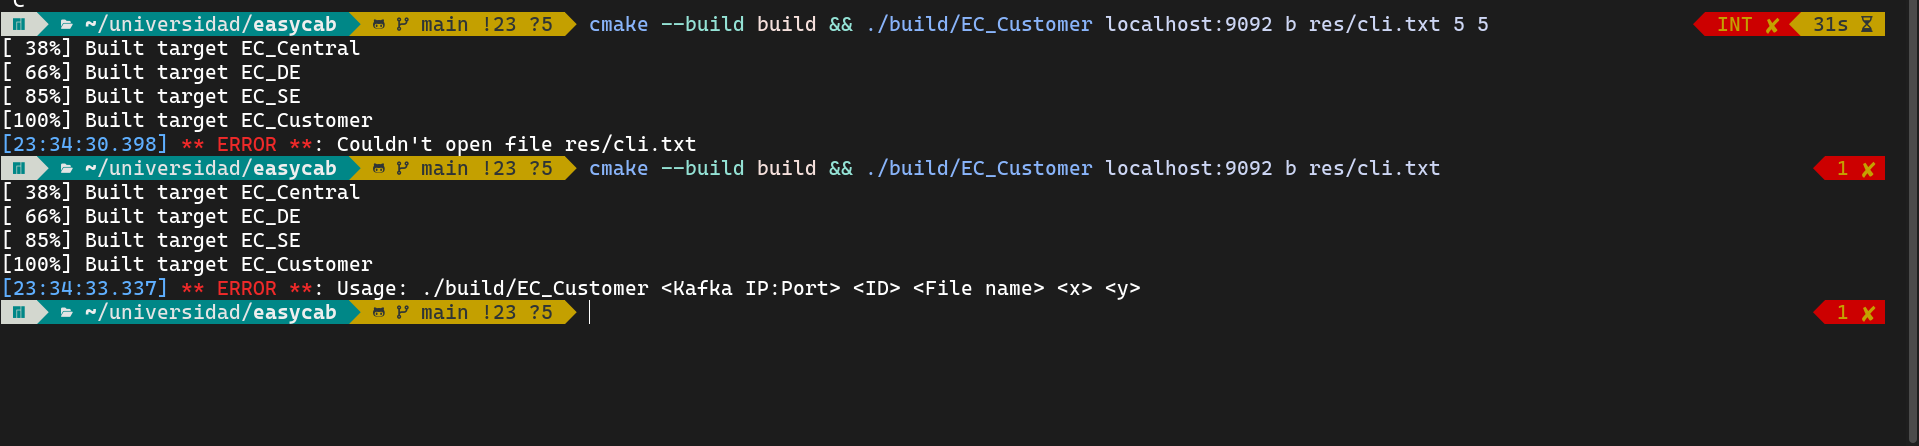
\includegraphics{img3.png}
  }
  \caption{Ejemplos de ejecución erróneos.}
\end{figure}
\begin{figure}[h]
  \centering
  \adjustbox{width=\paperwidth,center}{
    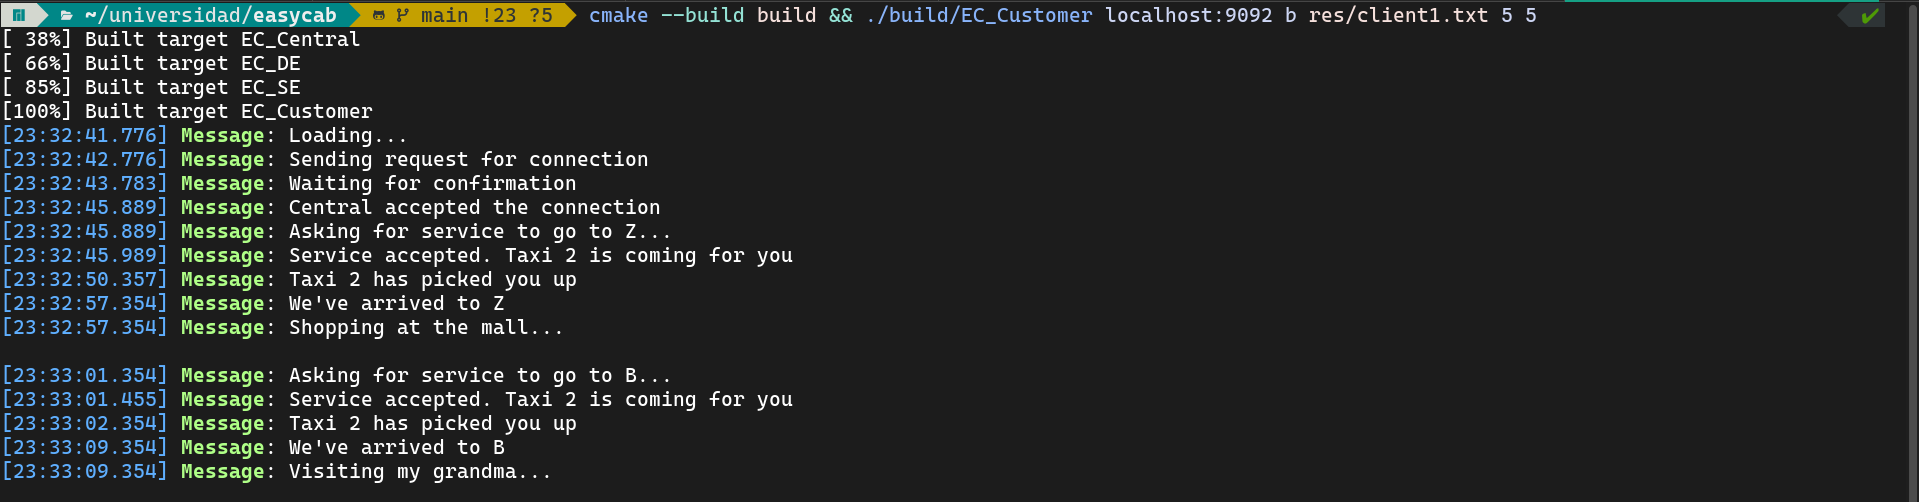
\includegraphics{img2.png}
  }
  \caption{Ejemplo de ejecución satisfactorio.}
\end{figure}

\clearpage
\subsection{EC\_SE}
Este es otro componente relativamente sencillo, si no tenemos en cuenta su interfaz gráfica. Consta de dos hilos de ejecución:
\begin{enumerate}
  \item \textbf{Principal}: Se encargará de comprobar los argumentos de entrada y de inicializar el sistema. Una vez todo esté listo
        (incluida la conexión con el taxi), creará el segundo hilo y se quedará a cargo de la interfaz gráfica.
  \item \textbf{Comunicación con el taxi}: Se encargará de la comunicación con el taxi: A cada segundo enviará un mensaje
        a través del socket informando de si se puede o no mover y por qué (se entenderá más adelante), acto seguido leerá
        un mensaje del taxi indicando si este se encuentra parado o no (por razones ajenas al sensor, como si no tiene ningún servicio que atender).
\end{enumerate}
Ambos hilos se comunican a través de variables globales y herramientas de control de hilos (mutexes en este caso). \par
\subsubsection{Parámetros}
Este programa recibirá solo un parámetro de entrada: la dirección del socket de escucha del taxi. \par
\subsubsection{Aspectos relevantes}
Este componente es responsable de que el sistema sea relativamente síncrono. Aunque no afecta al progreso del sistema y este podría
funcionar completamente asíncrono, las comunicaciones del sensor con el taxi están sincronizadas con los segundos reales. Esto
se ha añadido meramente como curiosidad. \par
En cada ocasión que el usuario indique al sensor que el taxi debe pararse, el hilo principal subirá un contador a la cantidad de
segundos que debe esperar el taxi. Por otro lado, aprovechando que el segundo hilo realiza una iteración cada segundo, será este
el encargado de ir reduciendo este contado hasta llegar a 0 de nuevo.
\subsubsection{Ejemplos de ejecución}
Las imágenes siguientes conforman un único proceso de ejecución del programa:
\begin{figure}[h]
  \centering
  \adjustbox{width=\paperwidth,center}{
    
\includegraphics{img4.png}
  }
\end{figure}
\begin{figure}[h]
  \centering
  \adjustbox{width=\paperwidth,center}{
    
\includegraphics{img5.png}
  }
\end{figure}
\begin{figure}[h]
  \centering
  \adjustbox{width=\paperwidth,center}{
    
\includegraphics{img6.png}
  }
\end{figure}
\begin{figure}[h]
  \centering
  \adjustbox{width=\paperwidth,center}{
    
\includegraphics{img7.png}
  }
\end{figure}
\begin{figure}[h]
  \centering
  \adjustbox{width=\paperwidth,center}{
    
\includegraphics{img8.png}
  }
\end{figure}
\clearpage
\subsection{EC\_DE}
Siguiendo en orden de complejidad, llega el turno de la digital engine. Este componente separa su ejecución en 4 hilos
justo después de comprobar que los parámetros de entrada son correctos:
\begin{itemize}
  \item \textbf{Pings}: Este hilo es prácticamente idéntico a su homónimo en el componente EC\_Customer. Se encargará de mandar
        pings a la central cada segundo para indicar que el cliente está activo.
  \item \textbf{Hilo de movimiento}: Este hilo entrará en un bucle infinito en el cual espera una señal de otro hilo para
        avanzar la posición del taxi hacia el destino y volver a esperar una señal.
  \item \textbf{Conexión con el sensor}: Se encargará de esperar la comunicación del sensor del taxi e indicar al hilo de movimiento
        cuando se puede mover. Se define que el taxi no se puede mover si la señal recibida por el sensor lo indica o si el hilo responsable
        la conexión con la central lo dictamina de esa manera (puede ser porque no haya servicio que atender o porque se haya ordenado al taxi que se detenga).
  \item \textbf{Conexión con la central}: Estará a la espera de mensajes de la central. Comunicará lo relevante al resto de hilos a través de variables globales.
        Así pues, este hilo es el que modifica las variables como objetivo (al que se moverá el hilo de movimiento) o \textit{canMove}, que indica
        al hilo de conexión con el sensor si puede enviar la señal de movimiento o no.
\end{itemize}
\subsubsection{Parámetros}
Este programa recibirá 4 parámetros de entrada:
\begin{enumerate}
  \item \textbf{Dirección de la central}: Ip del equipo donde se ha desplegado la central y el puerto de escucha que
        se ha configurado.
  \item \textbf{Dirección del broker de Kafka}: Dirección del broker de Kafka a utilizar para la autenticación de los taxis.
  \item \textbf{Puerto de escucha del sensor}: Puerto por el que se escuchará el sensor del taxi.
  \item \textbf{Id}: Identificador único del taxi, los valores admitidos son del 0 al 99.
\end{enumerate}
\subsubsection{Aspectos relevantes}
Este componente es el que más hilos contiene y más uso hace de erramientas de control de hilos:
\begin{itemize}
  \item \textbf{mutexes}: Se usan para sincronizar el acceso a las variables globales entre los distintos hilos.
  \item \textbf{condiciones}: Son las que usa el hilo de conexión con el sensor para indicar al hilo de movimiento cuando puede o no moverse.
        Además, se utiliza un juego de condiciones para sincronizar los hilos al comienzo de la ejecución: mientras que el hilo principal lleva a cabo
        el proceso de autenticación con el servidor central, el hilo de conexión con el sensor comienza a abrir el socket y preparar la escucha del sensor.
        Ambos hilos se informan mutuamente para indicar cuando pueden avanzar en sus tareas (por ejemplo, no se comenzará la autenticación hasta que se haya
        comprobado que se puede abrir el socket sin errores).
\end{itemize}
La autenticación con el servidor central (a través de sockets) utiliza el formato de tramas sugerido por los profesores: cada comunicación
que no es atómica (ACK, NACK, ENQ, etc) contará con un primer caracter STX al comienzo del buffer, un caracter ETX en la penúltima posición
del mismo y un caracter LRC al final del mensaje. Esto se hace para asegurar que los mensajes sean transmitidos correctamente. \par
\subsubsection{Ejemplos de ejecución}
\begin{figure}[h]
  \centering
  \adjustbox{width=\paperwidth,center}{
    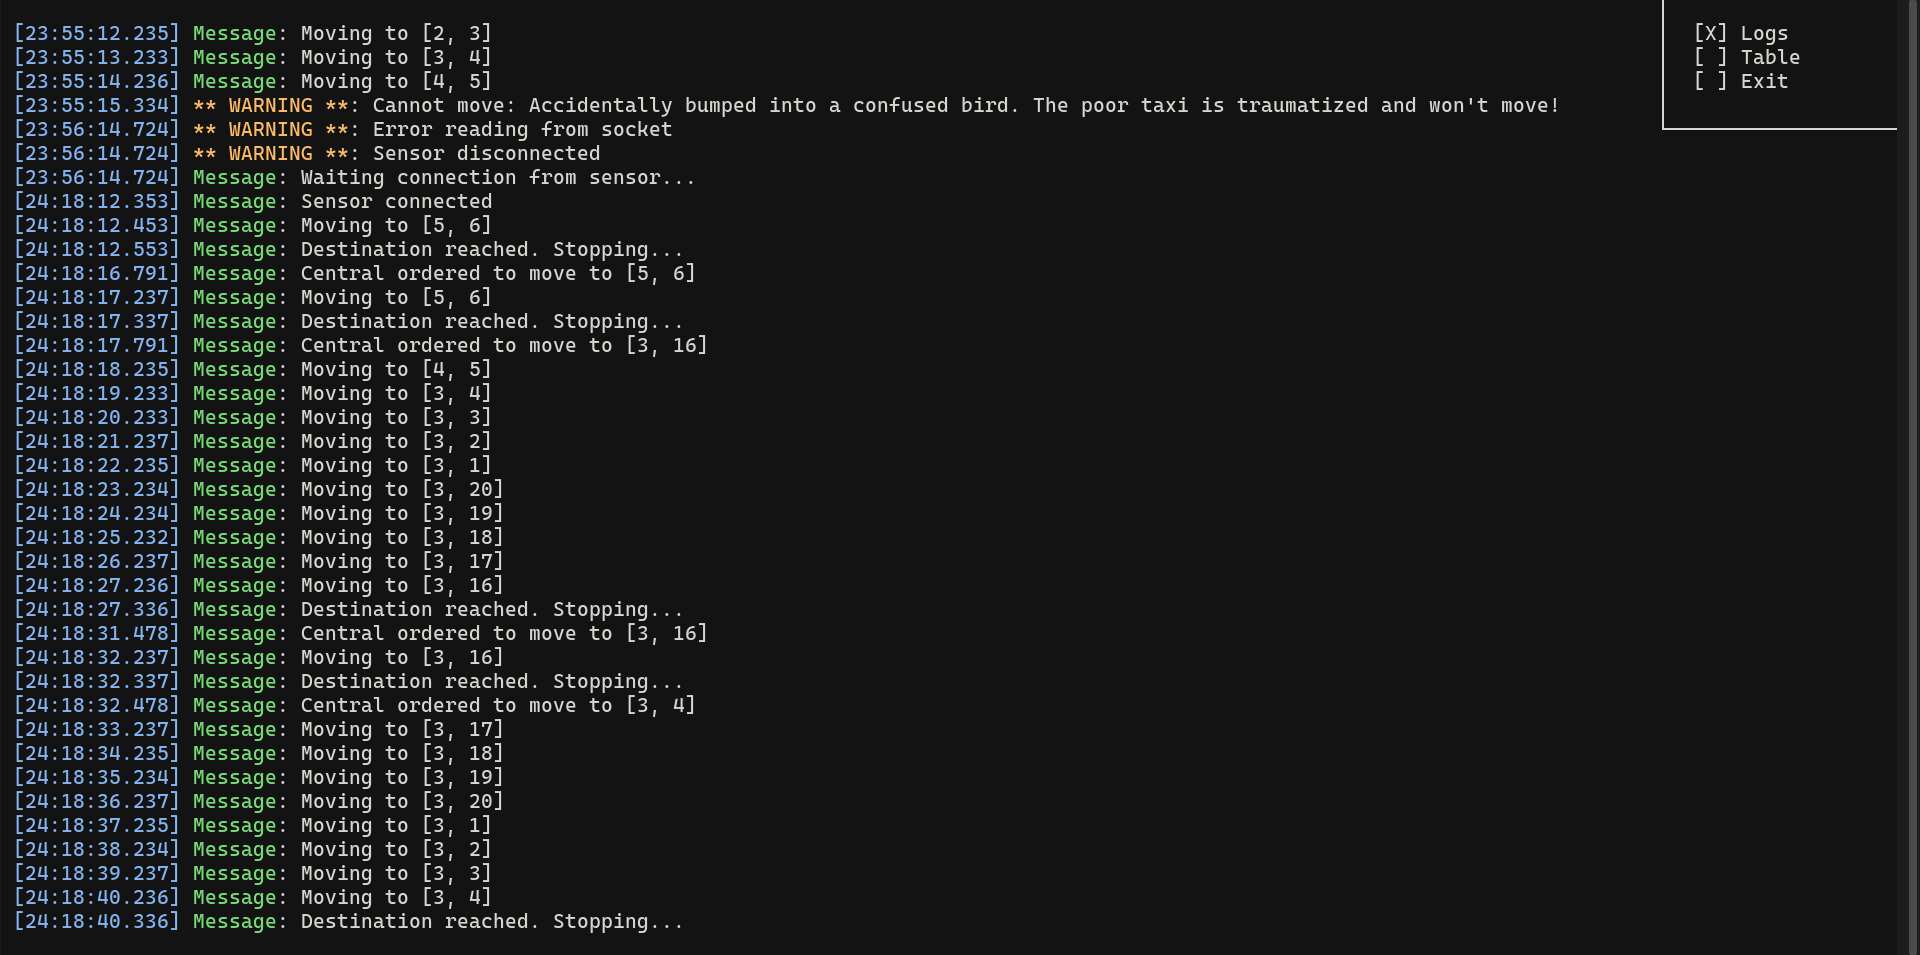
\includegraphics{img9.png}
  }
\end{figure}
\begin{figure}[h]
  \centering
  \adjustbox{width=\paperwidth,center}{
    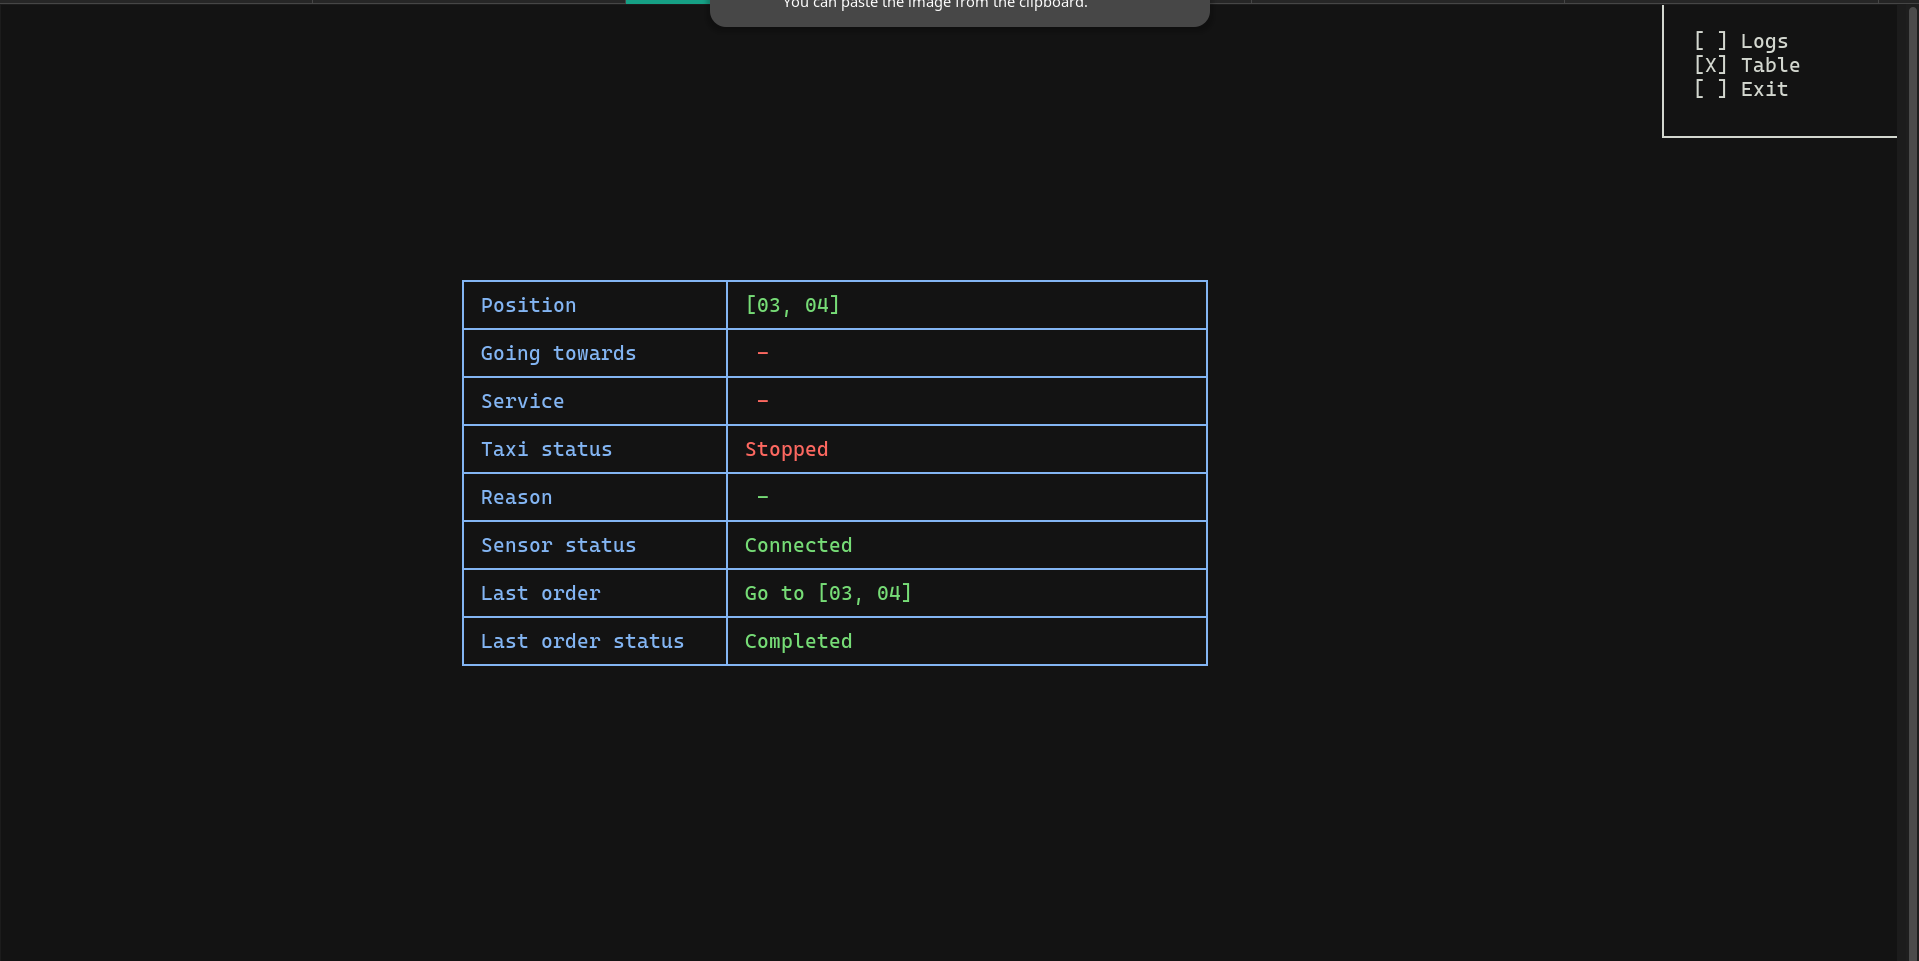
\includegraphics{img10.png}
  }
\end{figure}
\clearpage
\subsection{EC\_Central}
Este último componente es el encargado del control de todo el sistema. Nada más comenzar, se separará en tres procesos:
\begin{itemize}
  \item \textbf{Interfaz gráfica}: Se encargará de la comunicación con el usuario y de la presentación de los mensajes del sistema.
  \item \textbf{Socket}: Se encargará de escuchar peticiones de autenticación de los taxis a través de los sockets y de atenderlas.
  \item \textbf{Kafka}: Se encargará de escuchar peticiones a través de kafka y de atenderlas. Todo lo necesario será guardado
        en la base de datos.
\end{itemize}
\subsubsection{Parámetros}
Este programa recibirá tres parámetros de entrada:
\begin{enumerate}
  \item \textbf{Puerto de escucha}: Puerto a través del cual se escucharán las conexiones de los taxis para su autenticación.
  \item \textbf{Dirección del broker de Kafka}: Dirección del broker de Kafka a utilizar para la comunicación con el resto de componentes.
  \item \textbf{Dirección de la base de datos}: Dirección de servidor de gestión de la base de datos a utilizar durante la ejecución.
\end{enumerate}
\subsubsection{Aspectos relevantes}
Dentro del módulo de kafka, se creará un hilo separado que irá comprobando continuamente si hay clientes o taxis que han parado de
enviar pings. Si los hay, se notificará al hilo principal a través de un mensaje de kafka, como si de otro componente separado se tratase.
\par
Las localizaciones se leerán de un archivo "locations.csv" en la carpeta "res" del proyecto. Si no existe este archivo y se desea usar otra
ruta, se debe modificar la variable de entorno \textit{LOCATIONS\_PATH}. El formato esperado es el siguiente:
\begin{lstlisting}[language=bash]
  "A","1","1"
  "B","2","2"
  ...
\end{lstlisting}
\par
La central atenderá a la variable de entorno \textit{RESET\_DB} que indicará si se debe reiniciar la sesión y la bbdd (true) o no (false).
En realidad, solo comprobará si está definido y su valor es \textit{true}, en caso contrario dará por hecho que su valor es false.
\par
El módulo de kafka consta de un loop infinito en el que escucha una petición de kafka y la atiende. Casi cada posible motivo
tiene su propia función que sigue la siguiente estructura:
\begin{itemize}
  \item \textbf{Llamar al PROCEDURE de la base de datos correspondiente} (definidos en \textbf{initialize.sql})
  \item \textbf{Comprobar si la llamada se ha efectuado correctamente}
  \item \textbf{Informar de los resultados al usuario}
  \item \textbf{Comunicar los resultados al cliente o taxi que sea pertinente}
\end{itemize}
\subsubsection{Ejemplos de ejecución}
\begin{figure}[h]
  \centering
  \adjustbox{width=\paperwidth,center}{
    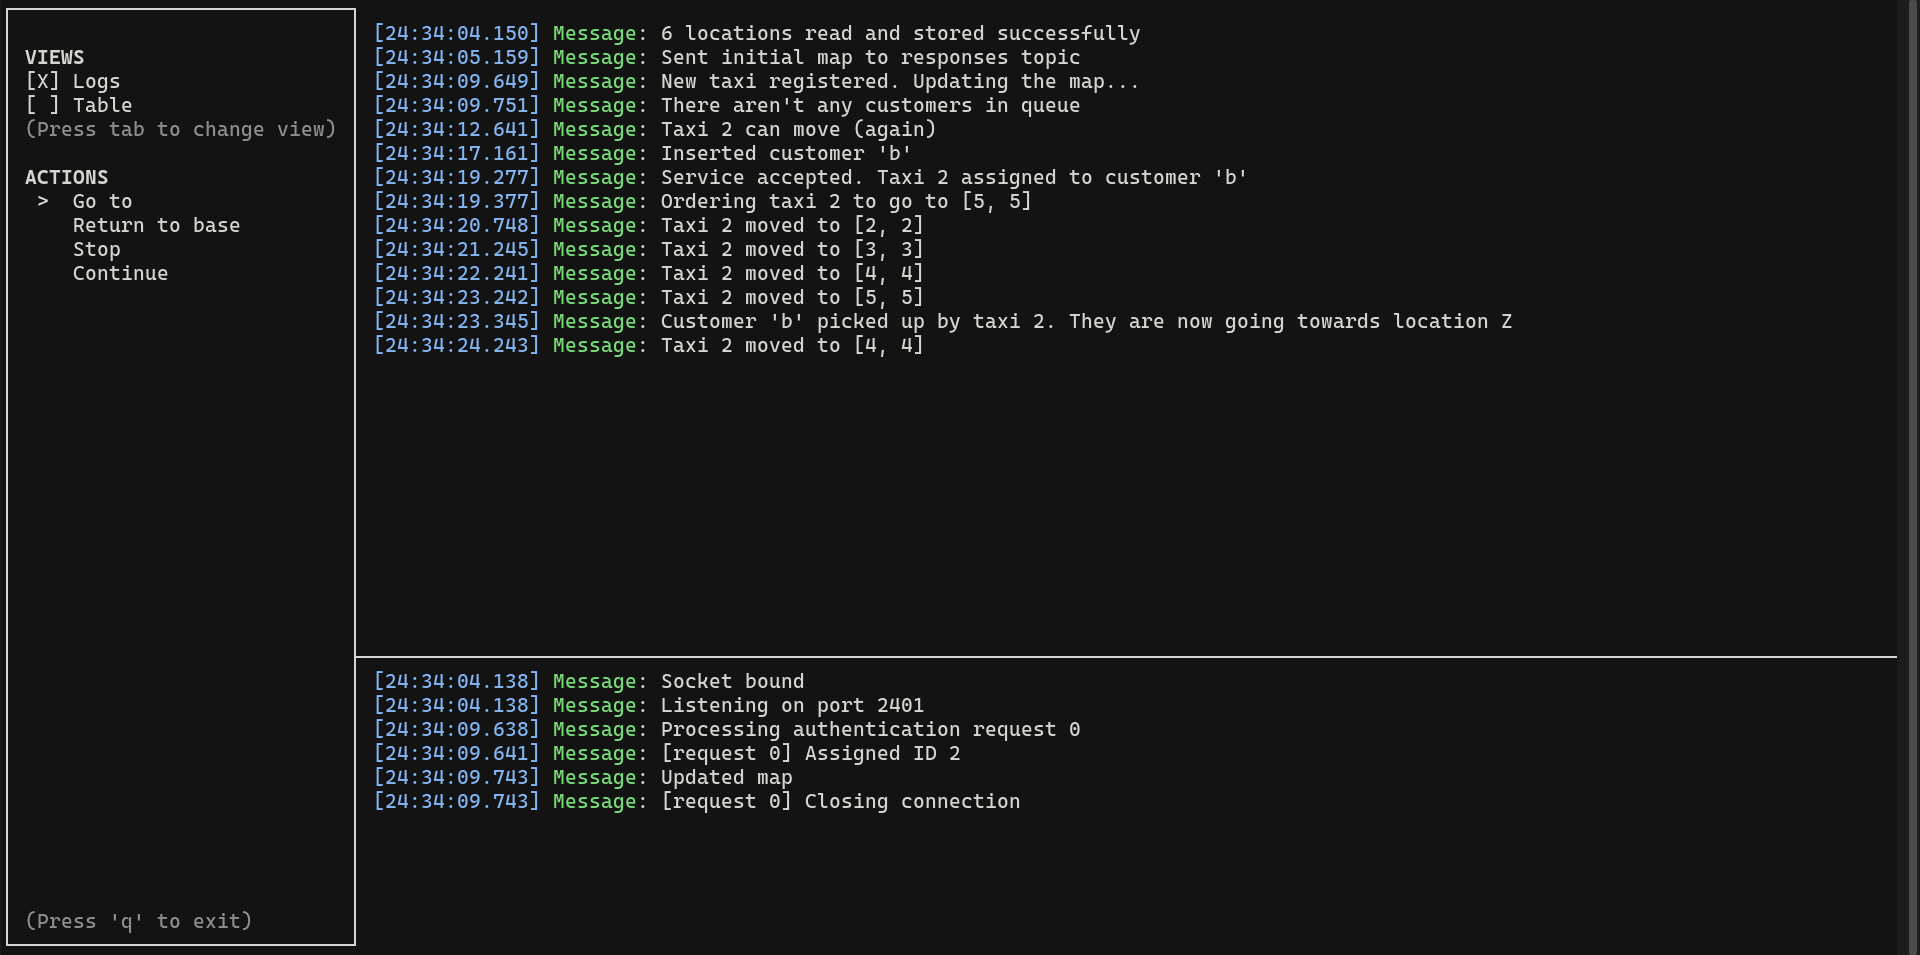
\includegraphics{img11.png}
  }
\end{figure}
\begin{figure}[h]
  \centering
  \adjustbox{width=\paperwidth,center}{
    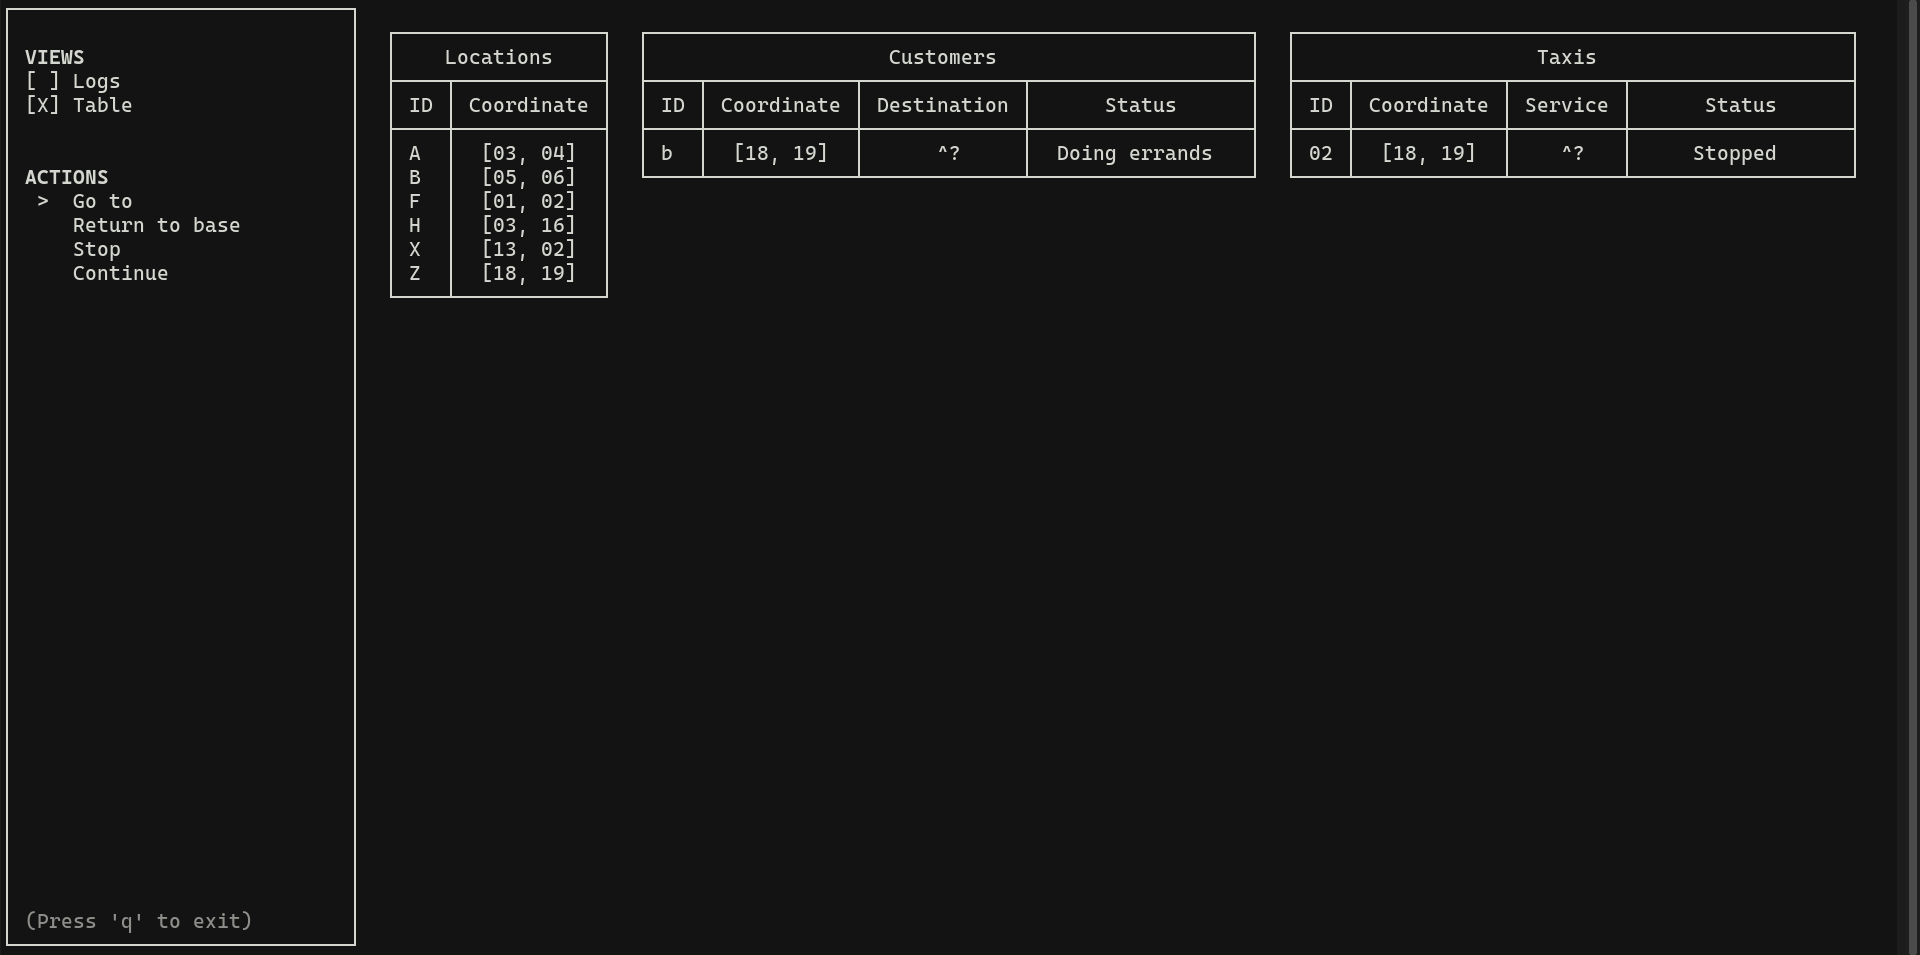
\includegraphics{img12.png}
  }
\end{figure}
\begin{figure}[h]
  \centering
  \adjustbox{width=\paperwidth,center}{
    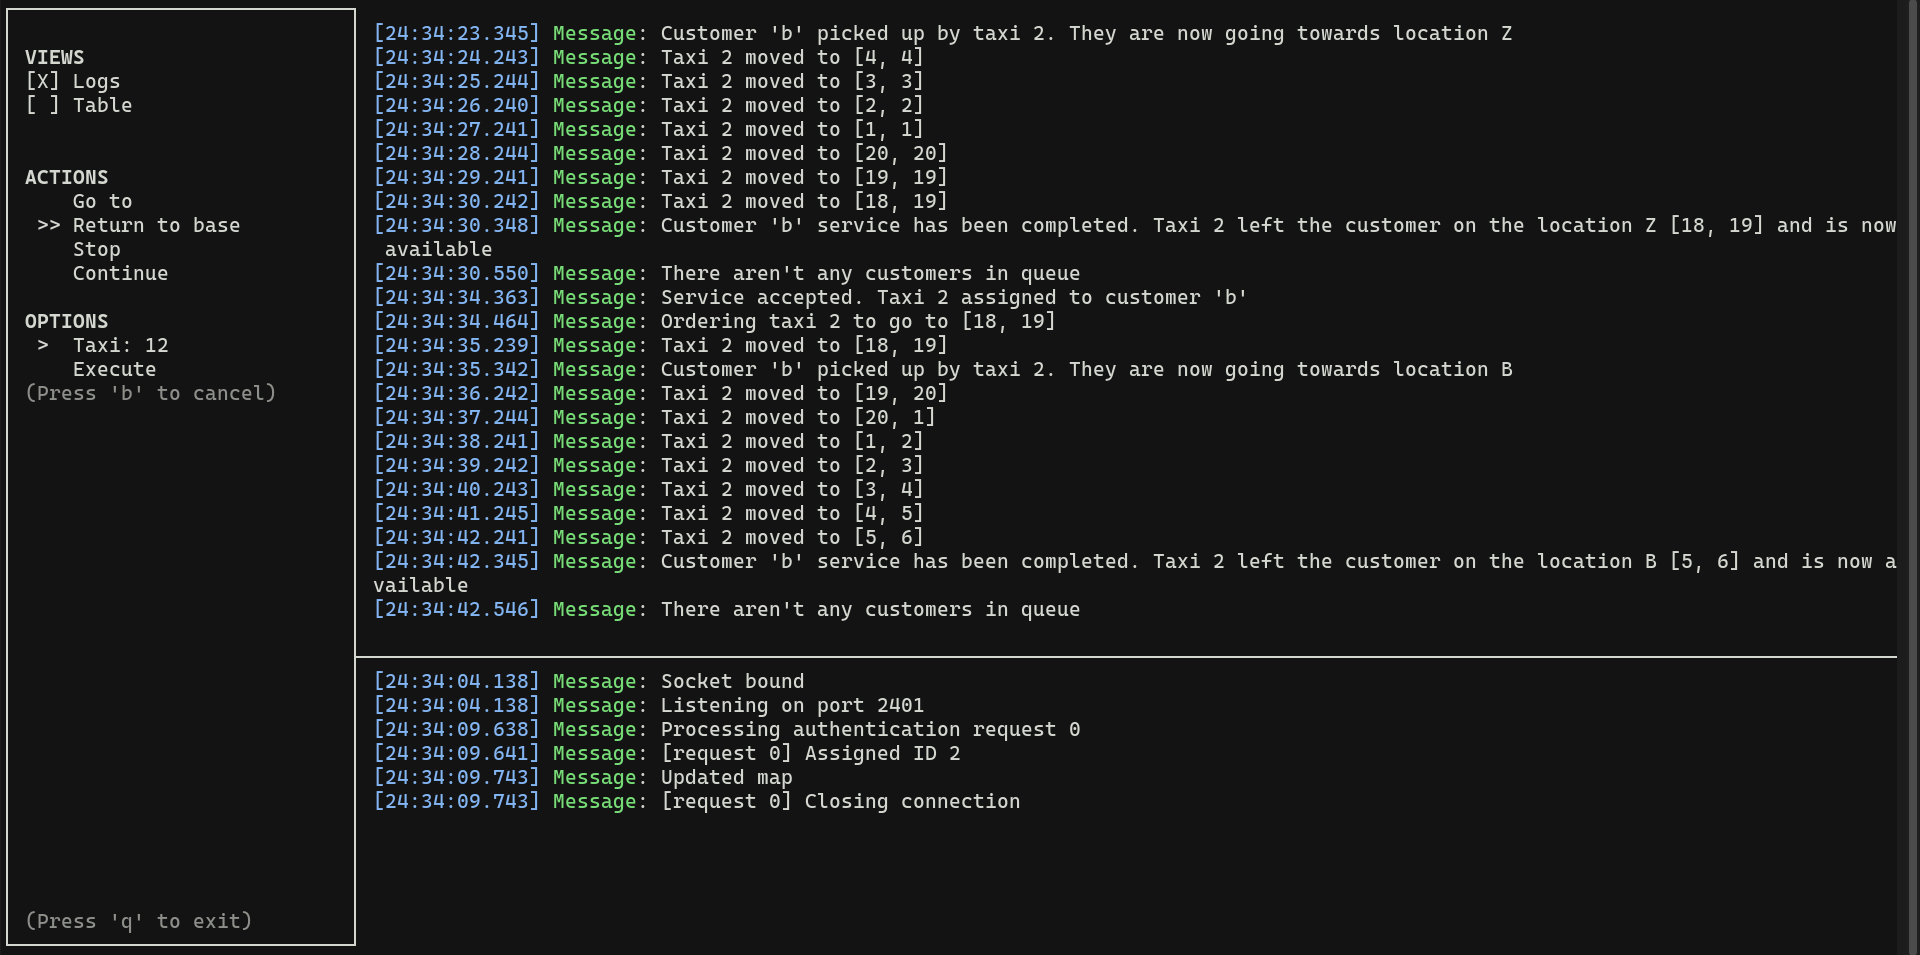
\includegraphics{img13.png}
  }
\end{figure}
\begin{figure}[h]
  \centering
  \adjustbox{width=\paperwidth,center}{
    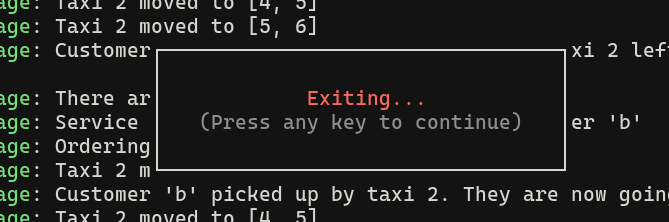
\includegraphics{img14.png}
  }
\end{figure}
\clearpage




\clearpage
\section{despliegue}
Como se comentó en la introducción, el despliegue está basado en Docker y, en menor medida, en Visual Studio.
\subsection{Componentes dockerizados}
\label{sec:componentes_docker}
Incluye todos los componentes a excepción de la interfaz gráfica.
Para desplegar cualquiera de ellos, el primer paso es crear y ejecutar un contenedor basado en la imagen
\href{https://hub.docker.com/repository/docker/abtb2/easycab_image/general}{easycab\_image}. \par

Puesto que las imágenes de Docker no son precisamente ligeras, para no depender de la conexión a internet lo ideal
será guardar la imagen previamente en formato \textit{.tar}:
\begin{lstlisting}[language=bash]
  docker save -o ./easycab_image.tar easycab_image
\end{lstlisting}

Para posteriormente instalarla localmente mediante el comando:

\begin{lstlisting}[language=bash]
  docker load -i ./easycab_image.tar
\end{lstlisting}

Si, por el contrario, no se dispone de una imagen previamente guardada, se puede descargar mediante el comando:

\begin{lstlisting}[language=bash]
  docker pull abtb2/easycab_image:latest
\end{lstlisting}
Una vez disponemos de la imagen, iniciaremos el contenedor con el comando:
\begin{lstlisting}[language=bash]
  sudo docker run --rm -e TERM=xterm-256color -ti easycab_image   
\end{lstlisting}
\footnote{
  La variable de entorno \textit{-e TERM=xterm-256color} es meramente estética. La mayoría de componentes cuentan
  con una interfaz gráfica de terminal basada en \textit{ncurses} y con colores. Si no se establece esta variable, simplemente
  toda la interfaz será en el mismo color, blanco y negro. A partir de aquí, incluirla o no ya es decisión del usuario.}

Es importante mencionar que, si el componente que se pretende ejecutar dentro del contenedor va a abrir un puerto de escucha,
es necesario añadir el argumento \textit{-p p1:p2}, donde la dirección ip\_host:p1 se conectará con el puerto p2 dentro del contenedor.
Es decir, si iniciamos el contenedor con el argumento \textit{-p 5000:8000} y, desde fuera del contenedor, tratamos de conectarnos a
localhost:\textbf{5000}, dentro del contenedor se recibirá una petición de conexión en el puerto \textbf{8000}. En cualquier caso, para evitar
confusiones, siempre es recomendable que ambos puertos sean el mismo. \par

Una vez iniciado el contenedor, nos encontraremos con un directorio de trabajo similar al del
\href{https://github.com/abtb2-ua/easycab}{proyecto}, con la diferencia de que en este caso, podremos encontrar la carpeta
\textit{build} con los archivos generados por cmake y los binarios compilados. Estos últimos son los que nos interesan. \par

Así pues, procederemos a ejecutar el componente deseado según las incidaciones en la sección de cada componente.

\subsection{Interfaz gráfica}
Para desplegar la interfaz gráfica, bastará con descargar la carpeta \textit{visual studio} del repositorio público y ejecutar
el archivo \textit{gui.sln} en un entorno de Windows. Esto abrirá una ventana de Visual Studio con el proyecto de la interfaz gráfica.
Una vez abierto, nos dirigiremos al administrador de paquetes de NuGet de la solución y instalaremos los paquetes requeridos para el
proyecto. A continuación, nos dirigiremos a propiedades del proyecto -> debugging -> argumentos adicionales y añadiremos la dirección al broker
de Kafka. Por último, ya podemos ejecutar el proyecto en modo release y ver el programa en acción.
\subsection{Kafka}
\label{sec:kafka}
\textbf{Requisitos}: tener java instalado en el sistema.
\textbf{Pasos}:
\begin{enumerate}
  \item \textbf{Descargar el archivo de Kafka}: \href{https://kafka.apache.org/downloads}{https://kafka.apache.org/downloads}
  \item \textbf{Extraer el archivo de Kafka}: \textit{tar -xzvf kafka\_2.8.1.tgz}
  \item \textbf{Iniciar el servidor de Zookeeper}: \textit{bin/zookeeper-server-start.sh config/zookeeper.properties}
  \item \textbf{Iniciar el servidor de Kafka}: \textit{bin/kafka-server-start.sh config/server.properties}
  \item \textbf{Desactivar windows defender o añadir una regla de firewall para permitir el acceso al puerto 9092}
        (desde el panel de control de seguridad de windows)
  \item \textbf{Inicializar los topics} (desde el directorio de Kafka):
        \begin{lstlisting}[language=bash]
    bin/kafka-topics.sh --bootstrap-server localhost:9092 --create --topic customer_responses &&
    bin/kafka-topics.sh --bootstrap-server localhost:9092 --create --topic taxi_responses &&
    bin/kafka-topics.sh --bootstrap-server localhost:9092 --create --topic map_responses &&
    bin/kafka-topics.sh --bootstrap-server localhost:9092 --create --topic requests
    \end{lstlisting}
\end{enumerate}
\subsection{Base de datos}
Terminamos explicando el despliegue de MySQL Server, que no tiene mucho misterio en realidad. Para desplegar la base de datos, lo
primero que tenemos que comprobar es que tengamos instalada la imagen de Docker mysql:latest. Esto se puede hacer descargándola
de Docker Hub o instalándola localmente, \hyperref[sec:componentes_docker]{como se comentó anteriormente}. Una vez instalada, bastará con
ejecutar el siguiente comando:
\begin{lstlisting}[language=bash]
  docker run --rm --name mysql-server -e MYSQL_ROOT_PASSWORD=1234 -v /ruta/initialize.sql:/docker-entrypoint-initdb.d/script.sql -p 3306:3306 mysql:latest
\end{lstlisting}
\textbf{¿Qué está haciendo este comando?} \par
Las flags \textbf{\textit{--rm}} y \textbf{\textit{--name}} no son imprescindibles, sirven para eliminar el contenedor cuando acabe su ejecución y para
etiquetarlo respectivamente. \par

Por el contrario, el siguiente argumento sí que es importante. \textbf{\textit{-e MYSQL\_ROOT\_PASSWORD=1234}}
define la contraseña para acceder a la bbdd y, dado que actualmente el código de la central no es flexible respecto a su uso (está definida
como una constante en el código fuente), se recomienda no cambiarla. \par

El siguiente parámetro \textbf{\textit{-v /ruta/initialize.sql:...}} indica que la base de datos cargará el archivo \textit{initialize.sql}
al inicializarse. Es importante tener acceso a este archivo (se encuentra en el
\href{https://github.com/abtb2-ua/easycab/blob/main/src/initialize.sql}{repositorio público} del proyecto) para desplegar la bbdd correctamente. \par

Por último, el parámetro \textbf{\textit{-p 3306:3306}} publica el puerto 3306 del contenedor en el host para poder recibir conexiones, como
se explicó en la sección de \hyperref[sec:componentes_docker]{componentes dockerizados}.
\clearpage
\textbf{Nota final}: debe notarse que el documento empieza siendo bastante trabajado y va desinflandose a medida que avanza.
A esto no tengo nada que hacer más que pedir disculpas. Recomiendo echarle un vistazo a las cabeceras (.h) del repositorio público
en github, donde están explicdas más a detalle cada una de las funciones que componen el proyecto.
\\
\\
Gracias por leer hasta el final.

\end{document}